\documentclass[border=5pt]{standalone}

\usepackage{tikz}
\usepackage{siunitx}

\usetikzlibrary{
    spath3,
    intersections,
    arrows,
    knots,
    calc,
    hobby,
    decorations.pathreplacing,
    shapes.geometric,
}

% ---------------- Global styles (safe for 'knots') ----------------
\tikzset{
    knot diagram/every strand/.append style={
        line cap=round,
        line join=round,
        ultra thick,
        black
    },
    every knot/.style={line cap=round,line join=round,very thick},
    strand/.style={line cap=round,line join=round,line width=3pt,draw=black},
    over/.style={preaction={draw=white,line width=6.5pt}},
% DO NOT set a global "every path" here; it breaks internal clip paths.
}


\begin{document}

% ====================================================================
% Trefoil (3_1)
% ====================================================================
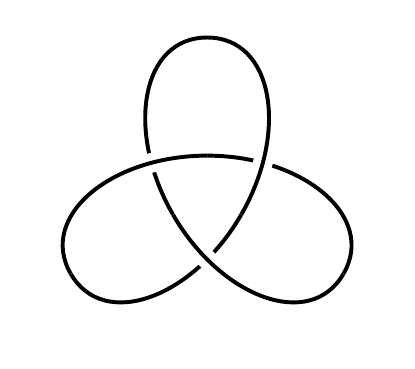
\begin{tikzpicture}[
    use Hobby shortcut,
    every path/.style={line width=1mm, white, double=black, double distance=.5mm}
]
\def\nfoil{3}
\draw ([closed]0,2)
foreach \k in {1,...,\nfoil} {
    .. ([blank=soft]90+360*\k/\nfoil-180/\nfoil:-.5) .. (90+360*\k/\nfoil:2)
};
\draw[use previous Hobby path={invert soft blanks,disjoint},double=black];
\end{tikzpicture}

\vspace{6mm}

% ====================================================================
% Trefoil (3_1) — 3 red / 3 blue
% ====================================================================
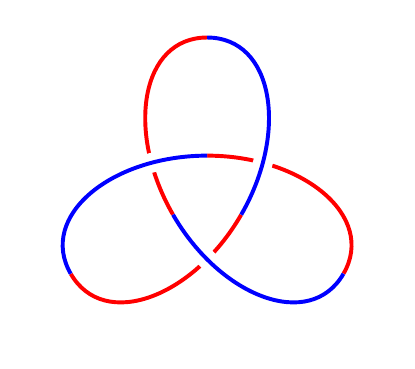
\begin{tikzpicture}[
    use Hobby shortcut,
    every path/.style={line width=1mm, white, double=red, double distance=.5mm}
]
\def\nfoil{3}
\draw ([closed]0,2)
foreach \k in {1,...,\nfoil} {
    .. ([blank=soft]90+360*\k/\nfoil-180/\nfoil:-.5) .. (90+360*\k/\nfoil:2)
};
\draw[use previous Hobby path={invert soft blanks,disjoint},double=blue];
\end{tikzpicture}

\vspace{6mm}

\par\medskip % or \bigskip
% ====================================================================
% Trefoil (3_1) — 1 blue component, 1 red component
% ====================================================================
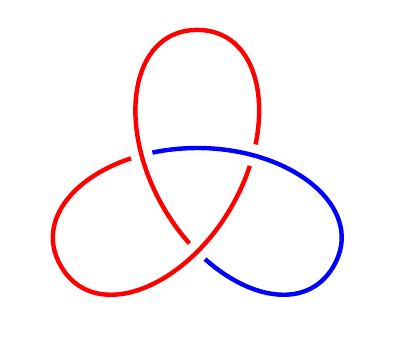
\begin{tikzpicture}[use Hobby shortcut]
\path[spath/save=trefoil]
([closed]90:2)
foreach \k in {1,...,3} { .. (-30+\k*240:.5) .. (90+\k*240:2) } (90:2);
\tikzset{
    every trefoil component/.style={ultra thick, draw, red},
    trefoil component 1/.style={blue},
    spath/knot={trefoil}{8pt}{1,3,5}
}
\end{tikzpicture}

\vspace{6mm}

\par\medskip % or \bigskip

% ====================================================================
% figure 8 (4_1)
% ====================================================================
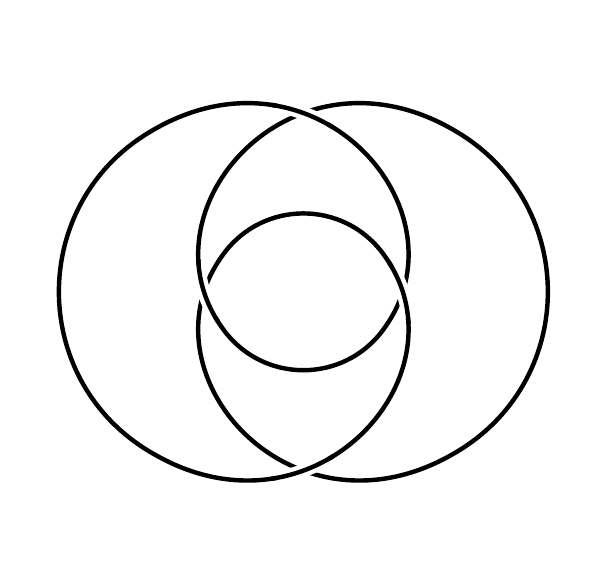
\begin{tikzpicture}[use Hobby shortcut]

\coordinate (P1) at (-2.0,  -2.0);  % start / close
\coordinate (P2) at (-2.0,  2.0);
\coordinate (P3) at ( 1, -0.5);
\coordinate (P4) at (-1, -0.5);
\coordinate (P5) at ( 2.0,  2.0);
\coordinate (P6) at ( 2.0, -2.0);
\coordinate (P7) at (-1,  0.5);
\coordinate (P8) at ( 1,  0.5);
\coordinate (P9) at (-2.0, -2.0);  % = P1 (smooth closed path)

\begin{knot}[
    consider self intersections,
    %draft mode=crossings,              % show crossing indices while tuning
    ignore endpoint intersections=true,
%    clip width=5pt, clip radius=3pt,
    flip crossing/.list={2,4,6,8,10,12,14}        % same over/under pattern as your snippet
]
\strand
([closed] P1)..(P2)..(P3)..(P4)..(P5)..(P6)..(P7)..(P8)..(P9);
\end{knot}

\end{tikzpicture}

\par\medskip % or \bigskip
% ====================================================================
% \(5_1\) cinquefoil
% ====================================================================
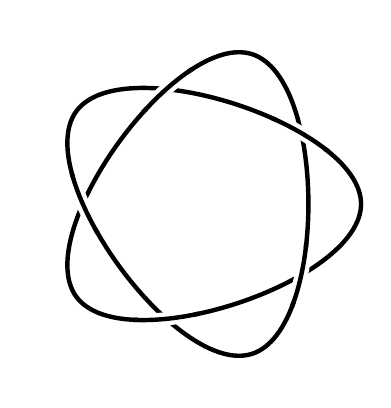
\begin{tikzpicture}
\begin{knot}[
    consider self intersections=true,
    %draft mode=crossings,
    flip crossing/.list={2,4,6,8,10}
% removed "only when rendering" and "show curve controls" (non-portable)
]
\strand (2,0)
.. controls +(0,1.0)   and +(54:1.0)  .. (144:2)
.. controls +(54:-1.0) and +(18:-1.0) .. (-72:2)
.. controls +(18:1.0)  and +(162:-1.0).. (72:2)
.. controls +(162:1.0) and +(126:1.0) .. (-144:2)
.. controls +(126:-1.0) and +(0,-1.0) .. (2,0);
\end{knot}
\end{tikzpicture}

\vspace{6mm}

\par\medskip % or \bigskip
% ====================================================================
% \(5_2\): Up Quark (SST sketch path)
% ====================================================================
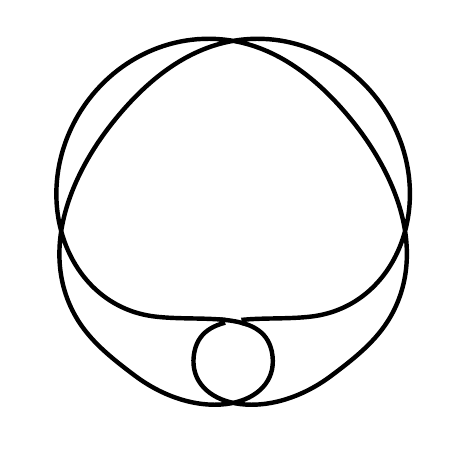
\begin{tikzpicture}[use Hobby shortcut]
\coordinate (P1) at (2, -1.5);
\coordinate (P2) at (1.5, 1);
\coordinate (P3) at (0, 2);
\coordinate (P4) at (-2, 1);
\coordinate (P5) at (-1, -1.5);
\coordinate (P6) at (0.5, -2);
\coordinate (P7) at (-1.25, -2.25);
\coordinate (P8) at (-2, -1.5);
\coordinate (P9) at (-1.5, 1);
\coordinate (P10) at (0, 2);
\coordinate (P11) at (2, 1);
\coordinate (P12) at (1, -1.5);
\coordinate (P13) at (-0.5, -2);
\coordinate (P14) at (1.25, -2.25);
\coordinate (P15) at (2, -1.5); % = P1

\begin{knot}[
    consider self intersections,
    clip width=5pt,
    clip radius=3pt,
    ignore endpoint intersections=true,
    flip crossing/.list={2,4,6,8,10,12,14,16,18}
% keep draft mode commented unless you want crossing indices
% draft mode=crossings
]
\strand
([closed] P1)..(P2)..(P3)..(P4)..(P5)..(P6)..(P7)..(P8)
..(P9)..(P10)..(P11)..(P12)..(P13)..(P14)..(P15);
\end{knot}

\SSTGuidesPoints{P}{15}
\end{tikzpicture}

\vspace{6mm}

\par\medskip % or \bigskip
% ====================================================================
% \(6_1\): Down Quark (Stevedore)
% ====================================================================
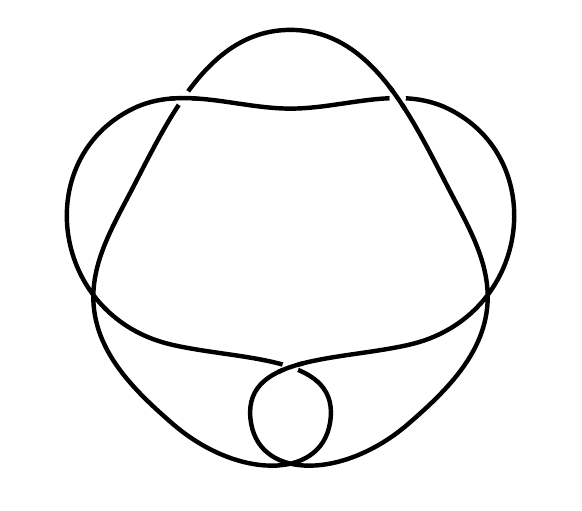
\begin{tikzpicture}[use Hobby shortcut]
\coordinate (P1)  at ( 0,  2);
\coordinate (P2)  at (-2,  2);
\coordinate (P3)  at (-1.5, -1);
\coordinate (P4)  at ( 0.5, -2);
\coordinate (P5)  at (-1.5,-2);
\coordinate (P6)  at (-2.5,-0.5);
\coordinate (P7)  at (-2, 1);
\coordinate (P8)  at ( 0,  3);
\coordinate (P9)  at ( 2, 1);
\coordinate (P10) at ( 2.5,-0.5);
\coordinate (P11) at ( 1.5,-2);
\coordinate (P12) at (-0.5, -2);
\coordinate (P13) at ( 1.5, -1);
\coordinate (P14) at ( 2,  2);
\coordinate (P15) at ( 0,  2); % = P1

\begin{knot}[
    consider self intersections,
    clip width=5pt,
    clip radius=3pt,
    ignore endpoint intersections=true,
    flip crossing/.list={2,4,6,8,10,12}
% draft mode=crossings
]
\strand
([closed] P1)..(P2)..(P3)..(P4)..(P5)..(P6)..(P7)..(P8)
..(P9)..(P10)..(P11)..(P12)..(P13)..(P14)..(P15);
\end{knot}

\SSTGuidesPoints{P}{15}
\end{tikzpicture}

\vspace{6mm}

\par\medskip % or \bigskip
% ====================================================================
% \(7_1\): septafoil
% ====================================================================
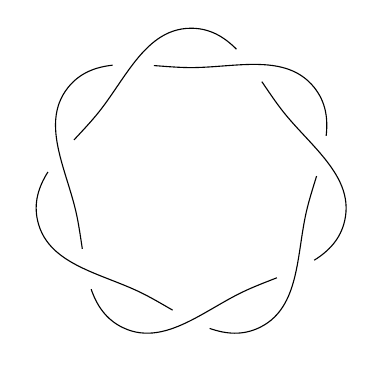
\begin{tikzpicture}[use Hobby shortcut]
\path[spath/save=sevenone]
([closed]90:2) foreach \k in {1,...,7} {
    .. (90-360/7+\k*720/7:1.5) .. (90+\k*720/7:2)
} (90:2);
\tikzset{
    every spath component/.style={draw},
    spath/knot={sevenone}{15pt}{1,3,...,15}
}
\end{tikzpicture}

\vspace{6mm}

\par\medskip % or \bigskip
% ====================================================================
% Hopf link
% ====================================================================
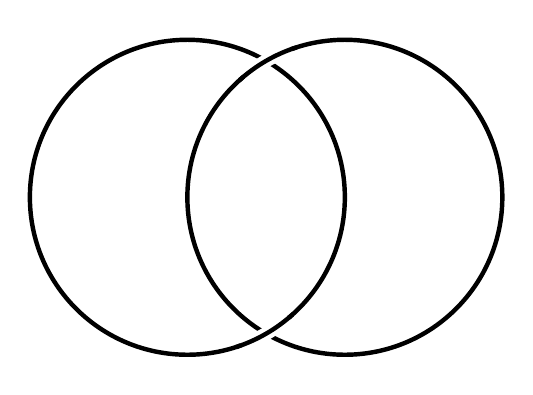
\begin{tikzpicture}
\begin{knot}[flip crossing=2]
\strand (1,0) circle[radius=2cm];
\strand[black] (-1,0) circle[radius=2cm];
\end{knot}
\end{tikzpicture}

\vspace{6mm}

\par\medskip % or \bigskip
% ====================================================================
% Borromean rings
% ====================================================================
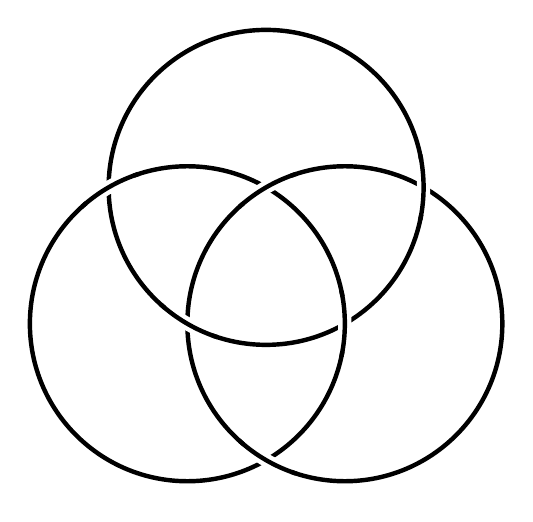
\begin{tikzpicture}
\begin{knot}[
    %draft mode=crossings,
    flip crossing/.list={3,4}]
\strand (1,0) circle[radius=2cm];
\strand[black] (-1,0) circle[radius=2cm];
\strand[black] (0,{sqrt(3)}) circle[radius=2cm];
\end{knot}
\end{tikzpicture}

\end{document}
